\section{Empirical Evaluation}
\label{sec:Empirical Evaluation}

 The validation of the MRs has been
designed to answer the following Research questions.

\begin{ResearchQuestion}
\label{ResearchQuestion_1}
Is our proposal effective in detecting errors in programs with constraints that implement scheduling problems?
\end{ResearchQuestion}
%Is our framework an effective way to find errors in Scheduling Problems?

The second concerns the extension of the proposal to other similar programs.

\begin{ResearchQuestion}
\label{ResearchQuestion_2}
Could our approach be useful to extend it to other programs that implement scheduling (in declarative languages or not)?
\end{ResearchQuestion}

%Finally, our third research question is related to the usefulness of our approach with respect to alternative approaches.
Finally, our third research question is related to new research findings.

\begin{ResearchQuestion}
\label{ResearchQuestion_3}
Has anything not originally proposed been discovered or detected?
% Alternativa:
% Have any extra results been discovered or detected?
\end{ResearchQuestion}
%Ahh, pues me alegro que me haga esa pregunta, que nosotros sepamos nunca se ha utilizado el intercambio de parámetros en una función hacer crear nuevos mutantes.
%¿Se necesita alguna herramienta nueva?

\subsection{Experiments}

We have conducted experiments with three classic scheduling problems coded in the constraint programming language \textit{MiniZinc} \cite{nethercote2007minizinc,marriott2014minizinc}.
Specifically, we start with the simplest example we have found,
Subsection \ref{subsubsec: Basic Scheduling Problem}, next two of the
most classic examples of programming with constraints, the \textit{Job
  Shop Problem}, Subsection \ref{subsubsect: Schedule for Jobshop
  problem}  \cite{xiong2022survey,fernandes2022energy} and, the
\textit{Moving Furniture Problem}, Subsection \ref{subsubsect: Moving
  Furniture Problem}.


In each case, we use one of the MRs that we have
presented in Section~\ref{sec:metamorfic_relations}.
For each
MR,  we generate a
mutant of the original program using one of the mutation operators in
Section~\ref{sec:mutants}.
Then we try to check the MR with the original program and
the mutant. In both cases we make the same operation: for a given
input (a scheduling problem instance) $i_{i}$ we compute its solution
$o_{1}$, then we build a following-up input $i_{2}$ and its
corresponding output $o_{2}$. 
Next, we check that the MR
holds for the outputs of the original program, but not for the
mutant. That is, we check that the metamorphic relation is able
to detect the mutant.


% Next, we describe the proposed problems and their corresponding testing.


In MiniZinc, files with the extension \texttt{mzn} correspond to
codes, that is, our objects under testing. The extension \texttt{dzn}
corresponds to data, that corresponds to the inputs, in our case
scheduling problem instances.
All examples, the code, and the inputs are public available in the
following GitHub link:
\url{https://github.com/LuisLlana/metamorphic_testing_constrints}.

\subsubsection{Basic Scheduling Problem}
\label{subsubsec: Basic Scheduling Problem}

In this problem, the resources are not taking into account, only the
duration and the precedence of the task.
The solution of this problem can be found in the MiniZinc repository.
In particular, is the file \lstinline{basic_sched.mzn} in
\url{https://github.com/MiniZinc/specialization-examples/tree/master/scheduling/basic}.
An example of the input of this program is the file
\lstinline{basic_sched.mzn}. This file defines the set of tasks:
\begin{lstlisting}
TASK = {FUNDS, SOLDIERS, DEFENSE, WEAPONRY_ART, ELITEARMY,
   RAW_MATERIALS, CRAFTSMEN, CASTING, BRICKS, WALL};
\end{lstlisting}
We do not need the concept of processor in this problem, so we can
assume that there is only one processor, so
the duration is given as a list
\begin{lstlisting}
duration = [10,10,25,25,10,20,15,20,10,20];
\end{lstlisting}
The precedence of the tasks is given in terms of a matrix
\begin{lstlisting}
        pre =
          [| FUNDS, SOLDIERS
           | FUNDS, RAW_MATERIALS
            ....
           | WALL, DEFENSE |];
\end{lstlisting}

Next, we are going to justify the convenience of the Metamorphic Relation
$MR2$. In order to achieve this, we are going to apply the
\textbf{MUT$\forall\exists$} to the following lines of the original code:

\begin{lstlisting}
constraint forall(i in PREC)
   (start[pre[i,1]] + duration[pre[i,1]] <= start[pre[i,2]]);
\end{lstlisting}

Thus, we obtain the following

% Sonia Comento la siguiente pq es la única con caption de su estilo
%\begin{lstlisting}[caption = {File: basic-MUT-forall-exists.mzn}, label={code.File: basic-MUT-forall-exists.mzn}]

\begin{lstlisting}
% Mutation: change 'forall' to 'exist'
constraint exits(i in PREC)
   (start[pre[i,1]] + duration[pre[i,1]] <= start[pre[i,2]]);
\end{lstlisting}

Then the original input $i_{1}$ corresponds to the scheduling problem
described above. Then we obtain the following-up input by adding an
inverse precedence. In the original input we have $\mathtt{FUNDS}\prec
\mathtt{SOLDIERS}$, then we define
$\mathtt{SOLDIERS}\prec_{2}\mathtt{FUNDS}$, formally
$\prec_{2}=(\prec\cup\{\mathtt{SOLDIERS},\mathtt{FUNDS}\})^{+}$. With
this new relation we obtain $i_{2}=mr_{2}(i_{1})$.

The code of the original code \lstinline{basic.mzn}, the mutant
\lstinline{basic-MUT-forall-exists.mzn}, the original input
\lstinline|basic.dzn|, and the following up input
\lstinline{basic-fu-cycle.dzn} are in the \texttt{MR2} folder of our
GitHub repository.

The original input has a solution, and the original
code establishes $o_{1}=\sol(i_{1})=85$. The follow-up adds a precedence constraint that forms a cycle in the
precedence graph. In fact, the original code detects that the problem
is unsatisfiable, that is $o_{2}=\sol(i_{2})=\infty$, as indicated in Figure
\ref{Fig:Add-inverse-precedence-a}. Therefore, the original code
\lstinline|basic.mzn| satisfies the MR
$MR2$
%\footnote{Formally we have not proved that \lstinline|basic.mzn|,
%we have not detected that it violates yet.}.

Instead, if we take the mutant \lstinline|basic-MUT-forall-exists.mzn|
the result is different. In this case, $o_{1}=o_{2}=25$ which violates $MR2$, as shown in
Figure \ref{Fig:Add-inverse-precedence-b}. So we can say that $MR2$
detects that \lstinline{basic-MUT-forall-exists.mzn} is a mutant.


\begin{figure}[!htb]
%\begin{minipage}{0.47\linewidth}
\begin{center}
\begin{tikzpicture}
 \node [mynode](I) at (-1.7,0.8) {$i_{1}$ (\lstinline|basic_sched.dzn|) };
 \node [mynode](O) at (-1.7,-0.8) {$o_{1}= 85$};
 \node [mynode](I') at (1.7,0.8) {$i_{2}$ (\lstinline|basic-fu-cycle.dzn|)};
 \node [mynode](O') at (1.7,-0.8) {$o_{2}=\infty$};

 \draw[myarrow](I) -- (O);
 \draw[myarrow](I') -- (O');

 \node [mylabel](code) at (0,0) {\lstinline|basic_sched.mzn|};

\end{tikzpicture}
\subcaption{Execution of the original code. $MR2$ is satisfied in this
case.}
\label{Fig:Add-inverse-precedence-a}
\end{center}
%\end{minipage}
%\begin{minipage}{0.05\linewidth}
%\end{minipage}
%\begin{minipage}{0.47\linewidth}
\begin{center}
\begin{tikzpicture}
 \node [mynode](I) at (-1.7,0.8) {$i_{1}$ (\lstinline|basic_sched.dzn|) };
 \node [mynode](O) at (-1.7,-0.8) {$o_{1}= 25$};
 \node [mynode](I') at (1.7,0.8) {$i_{2}$ (\lstinline|basic-fu-cycle.dzn|)};
 \node [mynodeRed](O') at (1.7,-0.8) {$o_{2}= 25$};

 \draw[myarrow](I) -- (O);
 \draw[myarrow](I') -- (O');

 \node [mylabel](code) at (0,0) {\lstinline|basicMUT-forall-exists.mzn|};

\end{tikzpicture}
\subcaption{Mutation execution}
\label{Fig:Add-inverse-precedence-b}
\end{center}
%\end{minipage}
\caption{Metamorphic relation MR2 and mutation execution}
\label{Fig:MR2_Add-inverse-precedence}
\end{figure}



In addition, using this example, we are going to show the convenience of the
metamorphic relation $MR1$.
All the programs and data are in the directory \lstinline{MR1} of our
GitHub repository.
The original program is in the file
\lstinline|basic-sched.mzn|
We apply the mutant operator
\textbf{MUT$\leq$} to the following line

\begin{lstlisting}
constraint forall(i in PREC)
   (start[pre[i,1]] + duration[pre[i,1]] <= start[pre[i,2]]);
\end{lstlisting}

to obtain
\begin{lstlisting}
constraint forall(i in PREC)
   (start[pre[i,1]] + duration[pre[i,1]] < start[pre[i,2]]);
\end{lstlisting}
The mutant is the file \lstinline|basic-MUT-<=-<.mzn|.

With respect to the input $i_{1}$ we are going to consider is the same as in the
previous case, it is in the file \lstinline|basic-sched.dzn|. The
following-up input $i_{2}$ is obtained as described in the MR.
It is in the file \lstinline{basic-fu-all-prec.dzn}.

If we consider the original program, we obtain $o_{1}=\sol(i_{1})=85$
and $o_{2}=\sol(i_{2})=165$, that is the duration of all
tasks. Therefore, the MR is satisfied in this case (Figure~\ref{Fig:MR1-Sequentility-all-tasks-a}).
Instead, if we consider the mutant, the solutions are
$o_{1}=\sol(i_{1})=89$ and $o_{2}=\sol(i_{2})=\infty$. Therefore, the
MR is violated (Figure~\ref{Fig:MR1-Sequentility-all-tasks-b}).



%En este caso se ha aplicado el operador de mutación  ERR definido en ~ \cite{puig2010equivalencias} para obtener el mutante.



\begin{figure}[!htb]
\begin{center}
%\begin{minipage}{0.47\linewidth}
\begin{center}
\begin{tikzpicture}
 \node [mynode](I) at (-1.7,0.8) {$i_{1}$ (\lstinline|basic_sched.dzn|) };
 \node [mynode](O) at (-1.7,-0.8) {$o_1= 85$};
 \node [mynode](I') at (2,0.8) {$i_{2}$ (\lstinline|basic-fu-all-prec.dzn|)};
 \node [mynode](O') at (2,-0.8) {$o_{2}= 165$};

 \draw[myarrow](I) -- (O);
 \draw[myarrow](I') -- (O');

 \node [mylabel](code) at (0,0) {\lstinline{basic_sched.mzn}};
\end{tikzpicture}
\subcaption{Original program execution}
\label{Fig:MR1-Sequentility-all-tasks-a}
\end{center}
%\end{minipage}
%\begin{minipage}{0.05\linewidth}
%\end{minipage}
%\begin{minipage}{0.47\linewidth}
\begin{center}
\begin{tikzpicture}
 \node [mynode](I) at (-1.7,0.8) {$i_{1}$ (\lstinline|basic_sched.dzn|)};
 \node [mynode](O) at (-1.7,-0.8) {$o_1= 89$};
 \node [mynode](I') at (2, 0.8) {$i_{2}$ (\lstinline{basic-fu-all-prec.dzn})};
 \node [mynodeRed](O') at (2,-0.8) {$o_{2}= \infty$};

 \draw[myarrow](I) -- (O);
 \draw[myarrow](I') -- (O');

 \node [mylabel](code) at (0,0) {\lstinline|basicMUT<=_<.mzn|};

\end{tikzpicture}
\subcaption{Mutation execution}
\label{Fig:MR1-Sequentility-all-tasks-b}
\end{center}
%\end{minipage}
\end{center}
\caption{Metamorphic relation MR1 and mutation execution}
\label{Fig:MR1-Sequentility-all-tasks}
\end{figure}



\subsubsection{Schedule for job shop problem}
\label{subsubsect: Schedule for Jobshop problem}

The job shop scheduling problem has been studied widely in research fields \cite{xiong2022survey} and its applications in different systems are relevant
\cite{fernandes2022energy,coelho2021thirty}.
The job shop scheduling model (our original program and input) is
taken from the MiniZinc
website\footnote{\url{https://www.minizinc.org/doc-2.5.5/en/modelling2.html},
  Listing 2.2.11}.
This problem describes a set of jobs, where each job is a sequence of tasks. The
tasks are mutually exclusive, so there cannot be two jobs executing the
same task at the same time. Formally, this problem can be seen that
there are several processors $P$ that have to execute a list of tasks
$T$.
The duration of any task depends on the processor that is executing it.
In
order to ensure the mutual exclusion there, for each task there is a
resource needed for its completion
$R=\{r_{t}\ |\ t\in T \}$. The function that assign resources is
$L(t)=\{r_{t}\}$.
% Sonia Comento la siguiente línea porque las restricciones
% de precedencia están intrísecas en el programa
%This problem does not consider precedence, it is the empty set: $\prec=\varnothing$.
With this problem we are going to study the convenience of the
MR $MR3$, all the code is in folder \lstinline|MR3| of
our GitHub repository. The original program is in the file
\lstinline|jobshop.mzn|, and the original data is in the file
\lstinline|jdata.dzn|, this is our original input $i_{1}$.
In this file, the duration of the tasks is
given in terms of matrix:
\begin{lstlisting}
d = [| 1, 4, 5, 3, 6
     | 3, 2, 7, 1, 2
     | 4, 4, 4, 4, 4
     | 1, 1, 1, 6, 8
     | 7, 3, 2, 2, 1 |];
\end{lstlisting}

Then we consider the following up input taking $c=99$, so the new
duration matrix is
\begin{lstlisting}
d = [| 100, 4, 5, 3, 6
     | 3, 2, 7, 1, 2
     | 4, 4, 4, 4, 4
     | 1, 1, 1, 6, 8
     | 7, 3, 2, 2, 1 |];
\end{lstlisting}
The modified file is \lstinline|jdata-fu+d.dzn|, this is our
following-up input $i_{2}$. When executing the original program, we
obtain $o_{1}=\sol(i_{1})=30$ and $o_{2}=\sol(i_{2})=126$. The
MR $MR3$ holds in this case (Figure~\ref{Fig:MR3. jobshop-forall-exists-1-a}).


We are going to consider two mutant operators. The first one is
\textbf{MUT$\forall\exists$}. We are going to apply
this operator to this part of code
\begin{lstlisting}
constraint
forall(i in JOB) (
 forall(j in TASK where j < last)
  (s[i,j]+d[i,j]<=s[i,enum_next(TASK,j)])
      /\ s[i,last] + d[i,last] <= end
 );
\end{lstlisting}
Since there are two \lstinline|forall| operators there are two
possible mutants
\begin{lstlisting}
constraint
 exists(i in JOB) (        % forall
  forall(j in TASK where j < last)
   (s[i,j] + d[i,j] <= s[i,enum_next(TASK,j)]) 
   /\ s[i,last] + d[i,last] <= end
 );
\end{lstlisting}
whose code is in the file \lstinline|jobshopMUT-forall-exists-1.mzn|,
and
\begin{lstlisting}
constraint
forall(i in JOB) (
 exists(j in TASK where j<last) % forall
  (s[i,j]+d[i,j]<=s[i,enum_next(TASK,j)]) 
  /\ s[i,last] + d[i,last] <= end
);
\end{lstlisting}
whose code is in the file \lstinline|jobshopMUT-forall-exists-2.mzn|.
The result of execution of the first mutant on the inputs are
$o_{1}=\sol(i_{1})=15$ and $o_{2}=\sol(i_{2})=15$
(Figure~\ref{Fig:MR3. jobshop-forall-exists-1-b}). Since $o_{1}\not<
o_{2}$, the MR $MR3$ does not hold and the mutant has
been detected. In the case of the second mutant, we obtain
$o_{1}=\sol(i_{1})=21$ and $o_{2}=\sol(i_{2})=21$, so the mutant is
also detected.

The other operator we can apply in this example is
\textbf{MUT$\wedge\vee$}. In order to it, we are going to focus on the
following
lines of the original code:
\begin{lstlisting}
constraint
 forall(j in TASK) (
  forall(i,k in JOB where i < k) (
   s[i,j] + d[i,j] <= s[k,j] \/
   s[k,j] + d[k,j] <= s[i,j]
  )
 );
\end{lstlisting}
By applying this mutant operator, we obtain
\begin{lstlisting}
constraint
 forall(j in TASK) (
  forall(i,k in JOB where i < k) (
   s[i,j] + d[i,j] <= s[k,j] /\
   s[k,j] + d[k,j] <= s[i,j]
  )
 );
\end{lstlisting}
The corresponding mutant is in the file
\lstinline|jobshopMUT-and-or.mzn|. Applying the inputs to this mutant
we obtain $o_{1}=\sol(i_{1})=0$ and $o_{2}=\sol(i_{2})=0$, so the mutant is
also detected.


\begin{figure}[h]
%\begin{minipage}{0.49\linewidth}
\begin{center}
\begin{tikzpicture}

 \node [mynode](I) at (-2,0.8) {$i_{1}$ (\lstinline|jdata.dzn|) };
 \node [mynode](O) at (-2,-1.4) {$o_{1}= 30$};
 \node [mylabel](code) at (0,-0.6) {\lstinline|jobshop.mzn|};
 \node [mynode](I') at (2,0.8) {$i_{2}$ (\lstinline|jdata-fu+d.dzn|)};
 \node [mynode](O') at (2,-1.4) {$o_{2} = 126$};

 \draw[myarrow](I) -- (O);
 \draw[myarrow](I') -- (O');

 \node [mynode,below= -0.2cm of I] (Icaption) {d[0,0] = 1};
 \node [mynode,below= -0.2cm of I'] (I'caption) {d[0,0] = 100};

\end{tikzpicture}
\subcaption{Original program execution}
\label{Fig:MR3. jobshop-forall-exists-1-a}
\end{center}
%\end{minipage}
%\begin{minipage}{0.49\linewidth}
\begin{center}
\begin{tikzpicture}

 \node [mynode](I) at (-2,0.8) {$i_{1}$ (\lstinline|jdata.dzn|) };
 \node [mynode](O) at (-2,-1.6) {$o_{1} = 15$};
 \node [mylabel](code) at (0,-0.7) {\lstinline|jobshopMUT-forall-exists-1.mzn|};
 \node [mynode](I') at (2,0.6) {I' (\lstinline|jdata-fu+d.dzn|)};
 \node [mynodeRed](O') at (2,-1.6) {$o_{2} = 15$};

 \draw[myarrow](I) -- (O);
 \draw[myarrow](I') -- (O');

 \node [mynode,below= -0.2cm of I] (Icaption) {d[0,0] = 1};
 \node [mynode,below= -0.2cm of I'] (I'caption) {d[0,0] = 100};

\end{tikzpicture}
\subcaption{Mutation execution}
\label{Fig:MR3. jobshop-forall-exists-1-b}
\end{center}
%\end{minipage}
\caption{Metamorphic relation MR3 and mutation execution}
\label{Fig:MR3. jobshop-forall-exists-1}
\end{figure}



\subsubsection{Moving Furniture Problem}
\label{subsubsect: Moving Furniture Problem}

The cumulative constraint is a global constraint with a set of jobs that require a certain number of different resources \cite{heinz2011explanations}.
Resources are uninterruptible and can be, for example, a set of machines or a group of workers with the same specialization.


A classic application of the cumulative constraint is the \textit{scheduling furniture moving} problem from Marriott and Stuckey \cite{marriott1998programming} page 112.
This constraint belongs to advanced modeling using global constraints \cite{Zhou2015} where
a global constraint captures a relation
that exists between a non-fixed number of variables, Handbook of Constraint Programming, chapter 6 \cite{GlobalConstraints}.



The scheduling furniture moving model given in the MiniZinc website\footnote{\url{https://www.minizinc.org/doc-2.5.5/en/predicates.html}, Listing 2.3.1},
describes a series of objects that must be moved (our set of tasks),
among which is a piano that requires a series of resources,
which are three handlers and two trolleys, in addition, the duration will be one hour.
The number of handlers and trolleys are limited.
Time to move all the furniture is also limited. This problem does not
consider processors, so we have to assume that there is one processor.

With this problem, we are going to study the convenience of the
$MR4$. All the code of this example is in the folder
\lstinline|MR4|.
The original program we are going to consider is
\lstinline|moving.mzn|.
The metamorphic relation MR4 establishes that if the execution of the
source input $i_{1}$ is satisfiable, and we increase the resources
required in the follow-up input \(i_{2}\) (for example, there are more
workers)
then $\sol(i_{2})\leq\sol(i_{1})$, that the required time (makespan) reduces.
That is, the increase in workers decreases the makespan,
but from a certain value it remains constant, as can be seen in the plots
in Figure~\ref{fig:more_workers}.

\begin{figure}\centering
  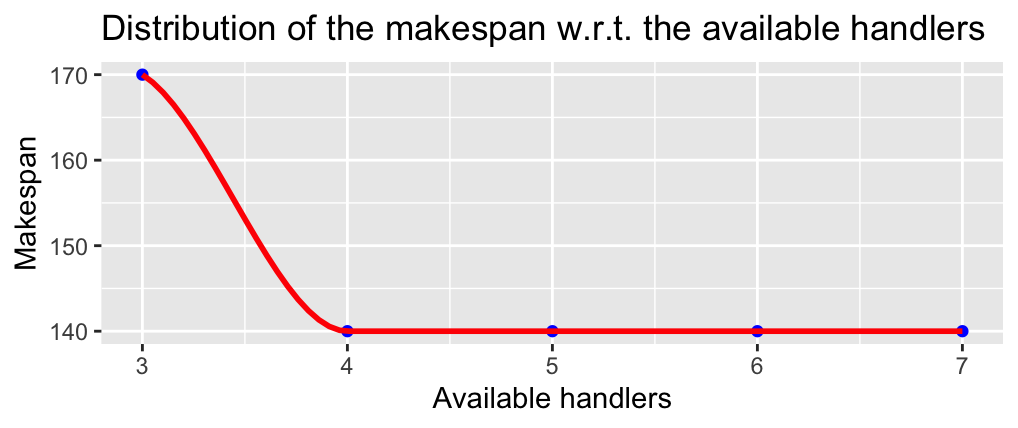
\includegraphics[scale=0.23]{Figures/1.png}
  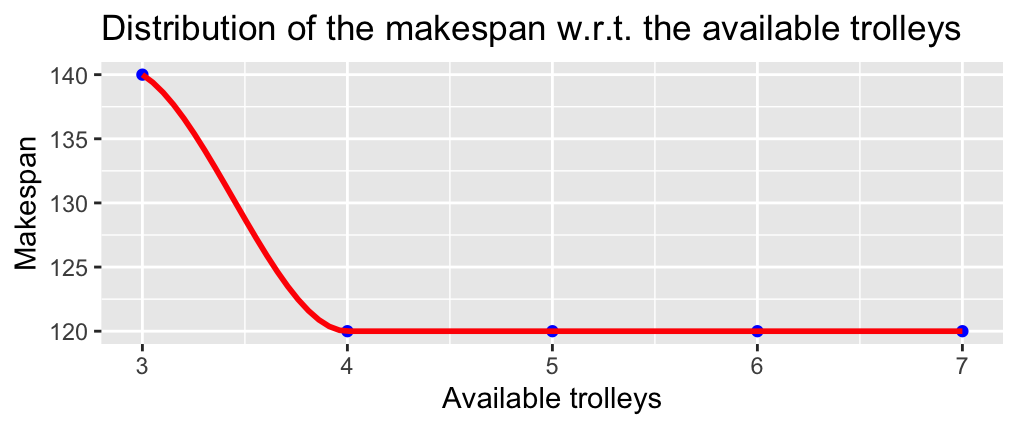
\includegraphics[scale=0.23]{Figures/2.png}
  \caption{Reduction of the makespan as the number of workers
    increases}
  \label{fig:more_workers}
\end{figure}

The original data of this program $i_{1}$ is in the file
\lstinline|moving.dzn|, whose contents are

\begin{lstlisting}
OBJECTS = {piano,fridge,doublebed,singlebed,wardrobe,chair1,chair2,table};

duration = [60,45,30,30,20,15,15,15];
handlers = [3,2,2,1,2,1,1,2];
trolleys = [2,1,2,2,2,0,0,1];

available_time = 180;
available_handlers = 4;
available_trolleys = 3;
\end{lstlisting}
We build the following-up input $i_{2}$ by increasing the number of
available handlers
\begin{lstlisting}
available_handlers = 40;
\end{lstlisting}
When executing the original program, we obtain $o_{1}=\sol(i_{1})=140$
$o_{2}=\sol(i_{2})=140$. The time does not increase, so the
MR $MR4$ holds in this case
(Figure~\ref{Fig:MR4 moving-con-mas-handlers-a}).

In order to generate the mutant, we are going to use
the mutant operator \textbf{MUT\(\Leftrightarrow\)}.
The original program contains the line
\begin{lstlisting}
constraint cumulative(start, duration, handlers, available_handlers);
\end{lstlisting}
where the first three parameters of cumulative are arrays of integer
variables. So we can obtain the line
\begin{lstlisting}
constraint cumulative(start, handlers, duration, available_handlers);
\end{lstlisting}
The mutant containing this modification is in the file
\lstinline{movingMUThandlers.mzn}.
when we execute the inputs with this mutant (in MiniZinc 2.6.4) we obtain  $o_{1}=\sol(i_{1})=\infty$
$o_{2}=\sol(i_{2})=\infty$. These data does not break the $MR4$
(Figure~\ref{Fig:MR4 moving-con-mas-handlers-a}).
But we have detected that there is a bug in the version 2.5.5 of MiniZinc.



\begin{figure}[!htb]
\begin{center}
\begin{tikzpicture}

 \node [mynode](I) at (-1.8,1) {$i_{1}$ (\lstinline|moving.dzn|) };
 \node [mynode](O) at (-1.8,-1.1) {$o_{1} = 140$};
 \node [mylabel](code) at (0,-0.3) {\lstinline|moving.mzn|};
 \node [mynode](I') at (1.8,1) {I' (\lstinline|moving+Handlers.dzn|)};
 \node [mynode](O') at (1.8,-1.1) {$o_{2} = 140$};

 \draw[myarrow](I) -- (O);
 \draw[myarrow](I') -- (O');

 \node [mynode,below= -0.2cm of I] (Icaption) {availableHandlers: 4};
 \node [mynode,below= -0.2cm of I'] (I'caption) {availableHandlers: 40};

\end{tikzpicture}
\subcaption{Original program execution}
\label{Fig:MR4 moving-con-mas-handlers-a}
\end{center}

\begin{center}
\begin{tikzpicture}
 \node [mynode](I) at (-2,1) {$i_{1}$ (\lstinline|moving.dzn|)};
 \node [mylabel](code) at (0,-0.3) {\lstinline|movingMUT-handlers.mzn|};
 \node [mynode](I') at (2,1) {$i_{2}$ (\lstinline|moving+Handlers.dzn|)};

 \node [mynodeRed](O) at (-2,-1.2) {$o_{1} = 140$};
\node (vers255) at (0,-1.2) {\textit{Vers 2.5.5.}};
 \node [mynodeRed](O') at (2,-1.2) {$o_{2}=\infty$};

 \node [mynode](O2) at (-2,-2.1) {$o_{1}=\infty$};
 \node [mynode](O'2) at (2,-2.1) {$o_{2}=\infty$};
 \node (vers255) at (0,-2.1) {\textit{Vers 2.6.4.}};

 \draw[myarrow](I) -- (O);
 \draw[myarrow](I') -- (O');

 \node [mynode,below= -0.2cm of I] (Icaption) {availableHandlers: 4};
 \node [mynode,below= -0.2cm of I'] (I'caption) {availableHandlers: 40};
\end{tikzpicture}
\subcaption{Mutation execution}
\label{Fig:MR4 moving-con-mas-handlers-b}
\end{center}
\caption{Metamorphic relation MR4 and mutation execution}
\label{Fig:MR4 moving-con-mas-handlers}
\end{figure}


In our tests in version 2.5.5. of the MiniZinc Figure
\ref{fig:ScreenShot_minizinc_2_5_5_bug}, the execution of source input
$i_{1}$
with four workers obtains a total time (makespan) of 140.
By increasing the number of workers, the makespan should have remained the same or reduced, but it was unsatisfiable and, this is not possible, Figure \ref{Fig:MR4 moving-con-mas-handlers}.



\begin{figure}[!htb]
    \centering
    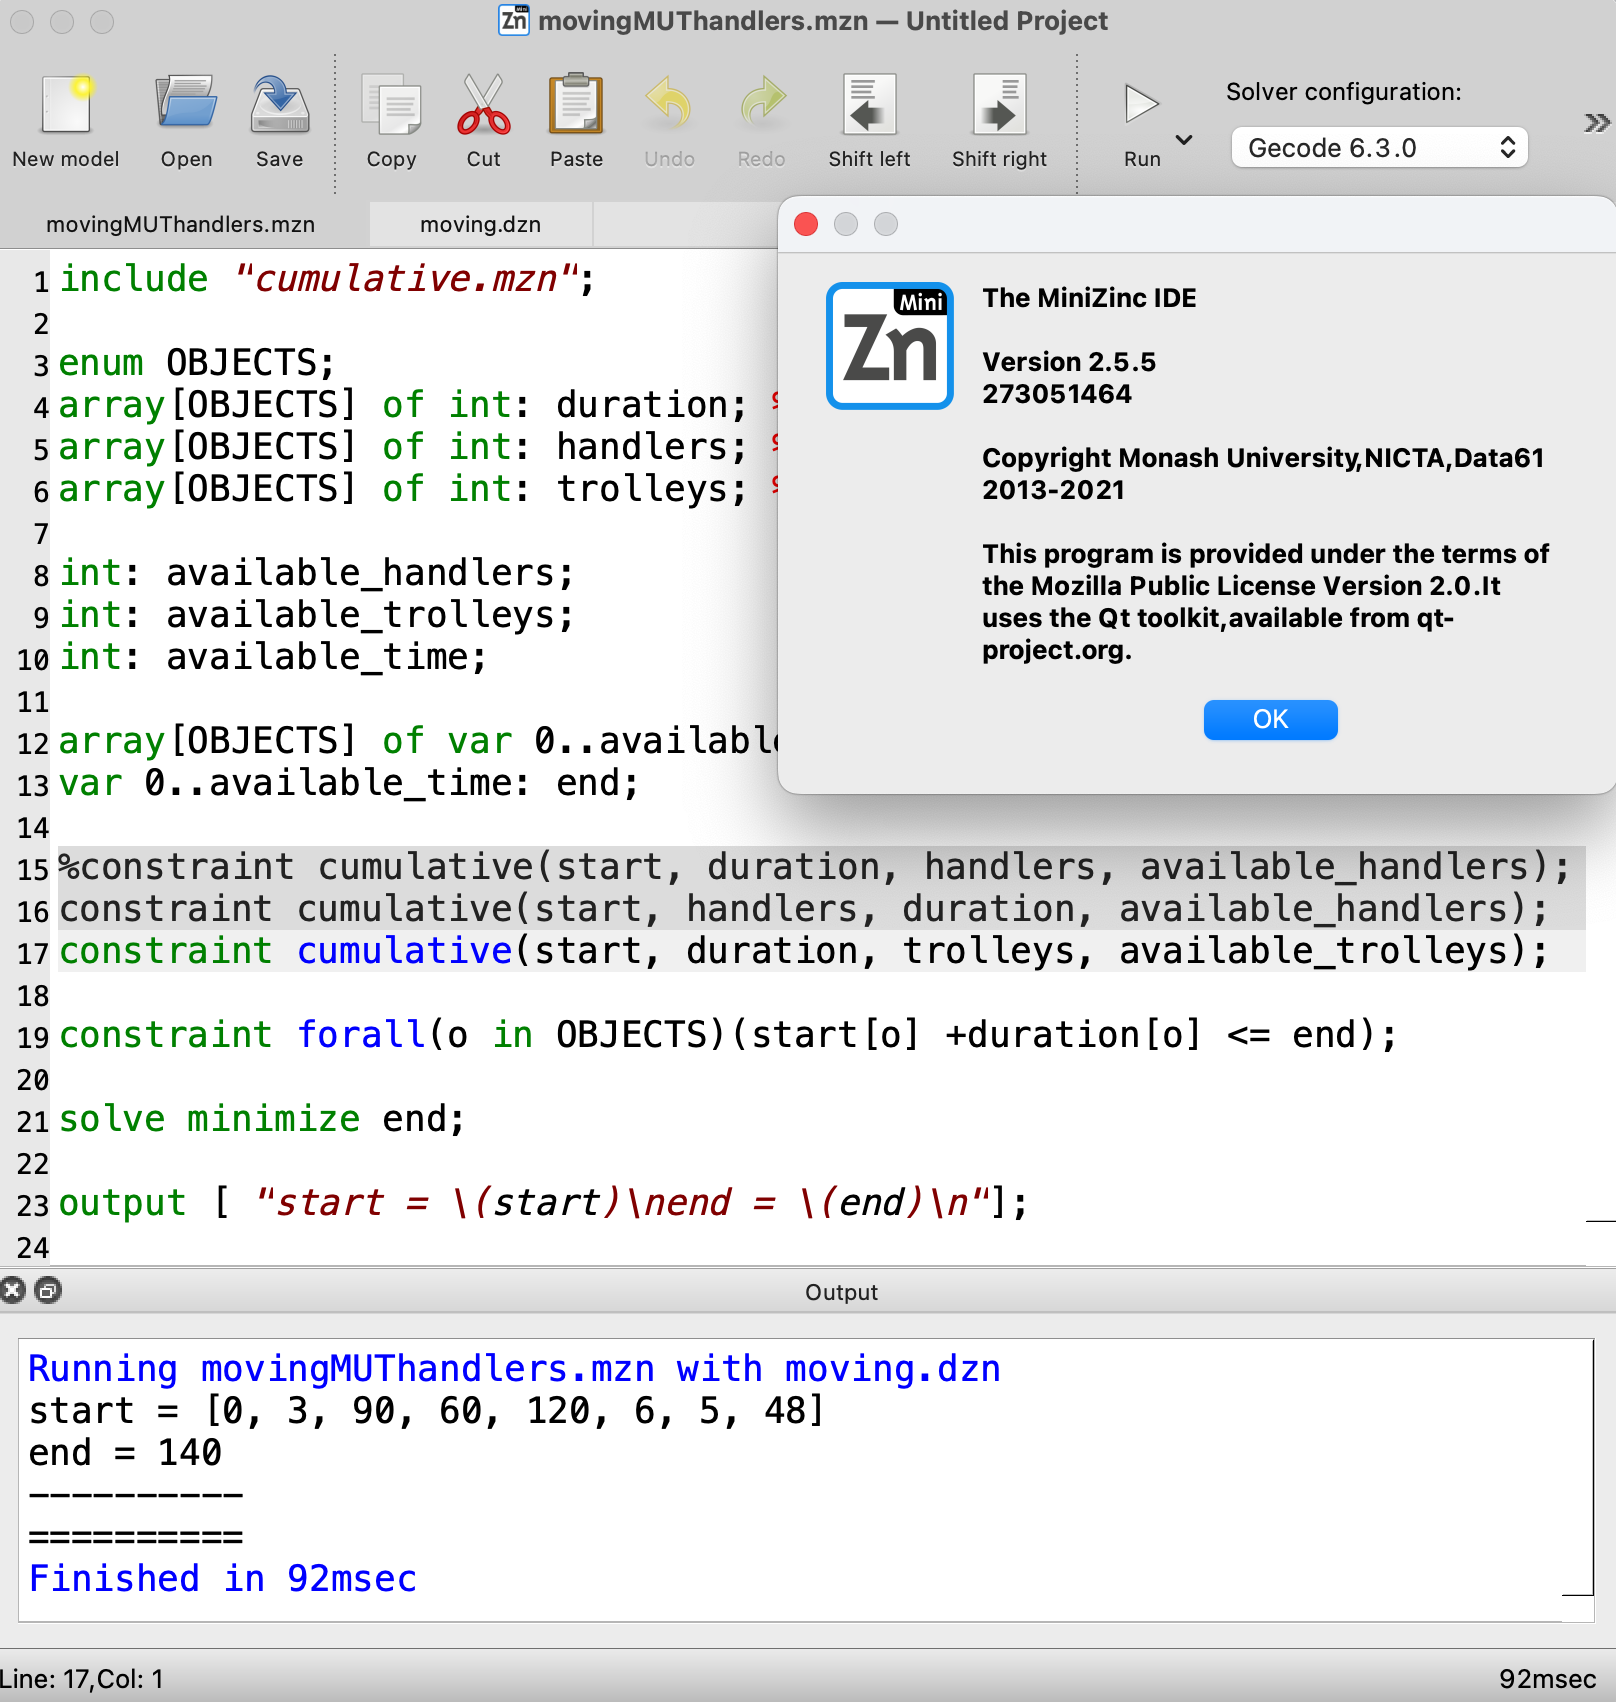
\includegraphics[scale = 0.28]{Figures/ScreenShot_minizinc_2_5_5_bug.png}
    \caption{Incorrect execution}
    \label{fig:ScreenShot_minizinc_2_5_5_bug}
\end{figure}


On the other hand, the execution of the same test in version 2.6.4. Figure \ref{fig:ScreenShot_minizinc_2_6_4_bug}
we obtain in both cases unsatisfactory.
This  demonstrates that version 2.5.5. had a bug that version 2.6.4. has already solved.

\begin{figure}[!htb]
    \centering
    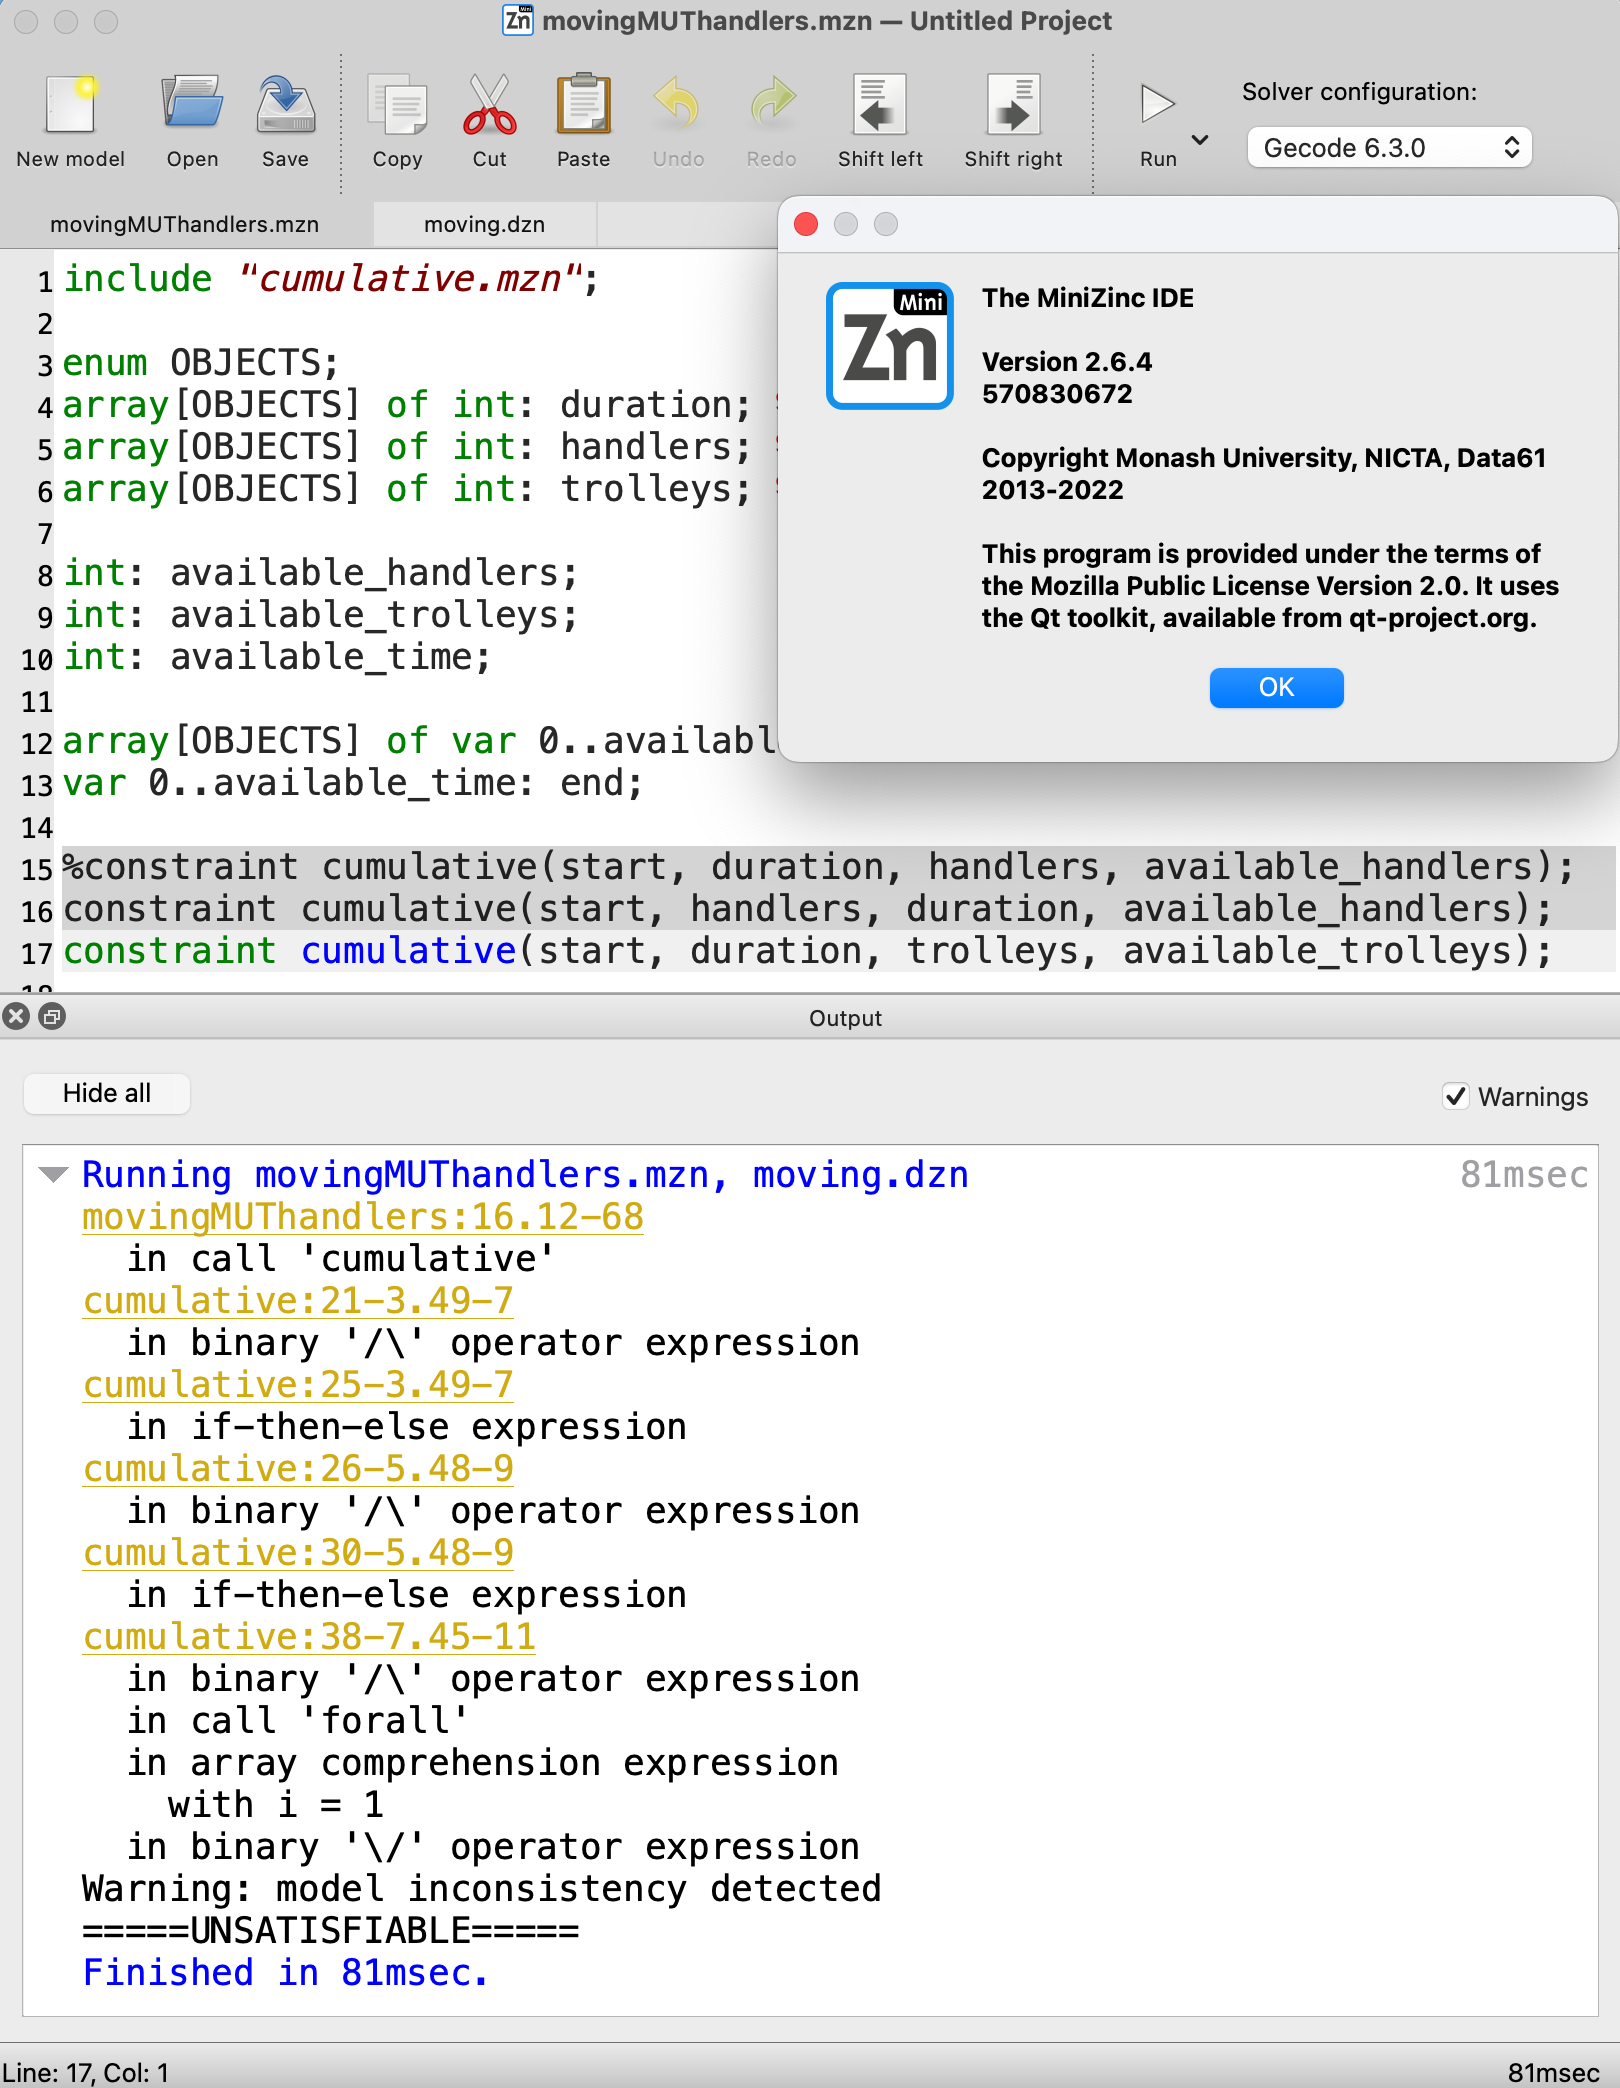
\includegraphics[scale = 0.28]{Figures/ScreenShot_minizinc_2_6_4_bug.png}
    \caption{Correct execution}
    \label{fig:ScreenShot_minizinc_2_6_4_bug}
\end{figure}


\subsection{Answers to the research questions}

According to the results obtained in the experiments conducted,
we consider the answer to Research Question 1 to be affirmative.
Our proposal has detected artificially
injected errors in the original code, as we have seen in
the previous sections. 


Regarding the answer to Research Question 2, we believe that it
is easily extendable, because MRs apply to test cases,
and scheduling problems follow a similar pattern in terms of the
information handled (restriction of tasks, time, resources, etc.).


Finally, regarding the answer to Research Question 3, collaterally,
we have detected a bug in the solver itself, through the metamorphic testing.
Therefore, potentially, although it needs more experiments,
it can also be useful
for testing constraint solvers. Likewise, when applying validation with
mutation testing, a new mutation operator related to logical
quantifiers (defined in Section \ref{s:mutOp}), exclusive for this type of
declarative languages, has been designed.
%%% \label{s:mutOp}
\subsection{Threats to validity}
In the following, we discuss the threats to the validity of the results of the
experiments presented in the previous section.
It should be noted that in our proposal the programs to be tested
represent the specifications of the problems to be solved, by being
implemented in a declarative language and solved with a constraint solver.
Therefore, as developers, we do not have as control over the solver
as for example on programs implemented in structured
or object-oriented languages.

On the other hand, scheduling problems have the search space is very large. 
For this reason, experiments have
been carried out focusing on several We are aware of the threat
to the validity of the scheduling problem, and we have designed
different implementation strategies for these problems.
We are aware of the threat to the validity of limiting
the scheduling problems to a small set of problems, but we think that
can be a representation of them, with the possibility of extension.

Regarding the threat to the validity of the implementation of the MRs,
since they are based on test case properties, they have been tested by hand
and with different data sets,  and a careful design has been made to
adapt each one to the type of problem to be solved and to the way in
which it has been implemented.

Finally, to validate the experiments, the mutation testing technique
was used to artificially introduce errors in the original code.
This has meant having to design mutation operators, as there is no
tool in the MiniZinc language for this purpose.



%%% Local Variables:
%%% mode: latex
%%% TeX-master: "../MT_scheduling"
%%% End:
